% Options for packages loaded elsewhere
\PassOptionsToPackage{unicode}{hyperref}
\PassOptionsToPackage{hyphens}{url}
\PassOptionsToPackage{dvipsnames,svgnames,x11names}{xcolor}
%
\documentclass[
  11pt,
]{article}

\usepackage{amsmath,amssymb}
\usepackage{iftex}
\ifPDFTeX
  \usepackage[T1]{fontenc}
  \usepackage[utf8]{inputenc}
  \usepackage{textcomp} % provide euro and other symbols
\else % if luatex or xetex
  \usepackage{unicode-math}
  \defaultfontfeatures{Scale=MatchLowercase}
  \defaultfontfeatures[\rmfamily]{Ligatures=TeX,Scale=1}
\fi
\usepackage{lmodern}
\ifPDFTeX\else  
    % xetex/luatex font selection
    \setmainfont[]{Times New Roman}
\fi
% Use upquote if available, for straight quotes in verbatim environments
\IfFileExists{upquote.sty}{\usepackage{upquote}}{}
\IfFileExists{microtype.sty}{% use microtype if available
  \usepackage[]{microtype}
  \UseMicrotypeSet[protrusion]{basicmath} % disable protrusion for tt fonts
}{}
\makeatletter
\@ifundefined{KOMAClassName}{% if non-KOMA class
  \IfFileExists{parskip.sty}{%
    \usepackage{parskip}
  }{% else
    \setlength{\parindent}{0pt}
    \setlength{\parskip}{6pt plus 2pt minus 1pt}}
}{% if KOMA class
  \KOMAoptions{parskip=half}}
\makeatother
\usepackage{xcolor}
\usepackage[margin=2.5cm]{geometry}
\setlength{\emergencystretch}{3em} % prevent overfull lines
\setcounter{secnumdepth}{5}
% Make \paragraph and \subparagraph free-standing
\makeatletter
\ifx\paragraph\undefined\else
  \let\oldparagraph\paragraph
  \renewcommand{\paragraph}{
    \@ifstar
      \xxxParagraphStar
      \xxxParagraphNoStar
  }
  \newcommand{\xxxParagraphStar}[1]{\oldparagraph*{#1}\mbox{}}
  \newcommand{\xxxParagraphNoStar}[1]{\oldparagraph{#1}\mbox{}}
\fi
\ifx\subparagraph\undefined\else
  \let\oldsubparagraph\subparagraph
  \renewcommand{\subparagraph}{
    \@ifstar
      \xxxSubParagraphStar
      \xxxSubParagraphNoStar
  }
  \newcommand{\xxxSubParagraphStar}[1]{\oldsubparagraph*{#1}\mbox{}}
  \newcommand{\xxxSubParagraphNoStar}[1]{\oldsubparagraph{#1}\mbox{}}
\fi
\makeatother


\providecommand{\tightlist}{%
  \setlength{\itemsep}{0pt}\setlength{\parskip}{0pt}}\usepackage{longtable,booktabs,array}
\usepackage{calc} % for calculating minipage widths
% Correct order of tables after \paragraph or \subparagraph
\usepackage{etoolbox}
\makeatletter
\patchcmd\longtable{\par}{\if@noskipsec\mbox{}\fi\par}{}{}
\makeatother
% Allow footnotes in longtable head/foot
\IfFileExists{footnotehyper.sty}{\usepackage{footnotehyper}}{\usepackage{footnote}}
\makesavenoteenv{longtable}
\usepackage{graphicx}
\makeatletter
\def\maxwidth{\ifdim\Gin@nat@width>\linewidth\linewidth\else\Gin@nat@width\fi}
\def\maxheight{\ifdim\Gin@nat@height>\textheight\textheight\else\Gin@nat@height\fi}
\makeatother
% Scale images if necessary, so that they will not overflow the page
% margins by default, and it is still possible to overwrite the defaults
% using explicit options in \includegraphics[width, height, ...]{}
\setkeys{Gin}{width=\maxwidth,height=\maxheight,keepaspectratio}
% Set default figure placement to htbp
\makeatletter
\def\fps@figure{htbp}
\makeatother
% definitions for citeproc citations
\NewDocumentCommand\citeproctext{}{}
\NewDocumentCommand\citeproc{mm}{%
  \begingroup\def\citeproctext{#2}\cite{#1}\endgroup}
\makeatletter
 % allow citations to break across lines
 \let\@cite@ofmt\@firstofone
 % avoid brackets around text for \cite:
 \def\@biblabel#1{}
 \def\@cite#1#2{{#1\if@tempswa , #2\fi}}
\makeatother
\newlength{\cslhangindent}
\setlength{\cslhangindent}{1.5em}
\newlength{\csllabelwidth}
\setlength{\csllabelwidth}{3em}
\newenvironment{CSLReferences}[2] % #1 hanging-indent, #2 entry-spacing
 {\begin{list}{}{%
  \setlength{\itemindent}{0pt}
  \setlength{\leftmargin}{0pt}
  \setlength{\parsep}{0pt}
  % turn on hanging indent if param 1 is 1
  \ifodd #1
   \setlength{\leftmargin}{\cslhangindent}
   \setlength{\itemindent}{-1\cslhangindent}
  \fi
  % set entry spacing
  \setlength{\itemsep}{#2\baselineskip}}}
 {\end{list}}
\usepackage{calc}
\newcommand{\CSLBlock}[1]{\hfill\break\parbox[t]{\linewidth}{\strut\ignorespaces#1\strut}}
\newcommand{\CSLLeftMargin}[1]{\parbox[t]{\csllabelwidth}{\strut#1\strut}}
\newcommand{\CSLRightInline}[1]{\parbox[t]{\linewidth - \csllabelwidth}{\strut#1\strut}}
\newcommand{\CSLIndent}[1]{\hspace{\cslhangindent}#1}

\usepackage{booktabs}
\usepackage{caption}
\usepackage{longtable}
\usepackage{colortbl}
\usepackage{array}
\usepackage{anyfontsize}
\usepackage{multirow}
\makeatletter
\@ifpackageloaded{caption}{}{\usepackage{caption}}
\AtBeginDocument{%
\ifdefined\contentsname
  \renewcommand*\contentsname{Table of contents}
\else
  \newcommand\contentsname{Table of contents}
\fi
\ifdefined\listfigurename
  \renewcommand*\listfigurename{List of Figures}
\else
  \newcommand\listfigurename{List of Figures}
\fi
\ifdefined\listtablename
  \renewcommand*\listtablename{List of Tables}
\else
  \newcommand\listtablename{List of Tables}
\fi
\ifdefined\figurename
  \renewcommand*\figurename{Figure}
\else
  \newcommand\figurename{Figure}
\fi
\ifdefined\tablename
  \renewcommand*\tablename{Table}
\else
  \newcommand\tablename{Table}
\fi
}
\@ifpackageloaded{float}{}{\usepackage{float}}
\floatstyle{ruled}
\@ifundefined{c@chapter}{\newfloat{codelisting}{h}{lop}}{\newfloat{codelisting}{h}{lop}[chapter]}
\floatname{codelisting}{Listing}
\newcommand*\listoflistings{\listof{codelisting}{List of Listings}}
\makeatother
\makeatletter
\makeatother
\makeatletter
\@ifpackageloaded{caption}{}{\usepackage{caption}}
\@ifpackageloaded{subcaption}{}{\usepackage{subcaption}}
\makeatother

\ifLuaTeX
  \usepackage{selnolig}  % disable illegal ligatures
\fi
\usepackage{bookmark}

\IfFileExists{xurl.sty}{\usepackage{xurl}}{} % add URL line breaks if available
\urlstyle{same} % disable monospaced font for URLs
\hypersetup{
  colorlinks=true,
  linkcolor={blue},
  filecolor={Maroon},
  citecolor={Blue},
  urlcolor={Blue},
  pdfcreator={LaTeX via pandoc}}


\author{}
\date{}

\begin{document}

\begin{titlepage}
    \noindent
    \begin{flushleft}
        \textbf{James Lewis} \\
    \end{flushleft}

    \vspace*{0.8cm}
    \centering

    \centering
    \vspace*{1.5cm}

    \includegraphics[width=0.42\textwidth]{Uni-Exeter-logo-portrait-1.png}\par\vspace{1.2cm}

    {\scshape\Large University of Exeter \par}
    \vspace{1.2cm}

    {\Huge\bfseries Long-Term Phytoplankton Disruption in the Gulf of Mexico: A Zonal Time-Series Analysis of the Deepwater Horizon Spill \par}
    \vspace{0.6cm}

    {\large Module Code: MTHM507 – Communicating Data Science\par}
    
    \vspace*{0.8cm}

    \small
    \noindent\rule{\textwidth}{0.4pt}
    \vspace{0.2cm}

    \textbf{Declaration of AI Assistance} \\
    I have used OpenAI’s ChatGPT tool in creating this report. \\

    AI-supported/AI-integrated use is permitted in this assessment. I acknowledge the following uses of GenAI tools in this assessment:

    \begin{itemize}\itemsep0pt \topsep0pt \parsep0pt
      \item Checking and debugging code
      \item Proofreading grammar and spelling
      \item Improving writing style and coherence
      \item Providing feedback on a draft
    \end{itemize}

    \vspace{-0.2cm}
    I declare that I have referenced use of GenAI outputs within my assessment in line with the University referencing guidelines.

\end{titlepage}

\renewcommand*\contentsname{Table of contents}
{
\hypersetup{linkcolor=}
\setcounter{tocdepth}{3}
\tableofcontents
}

\newpage

\section{Introduction}\label{introduction}

Phytoplankton are microscopic, photosynthetic organisms that form the
base of marine food webs and play a critical role in regulating the
global carbon cycle. Although they comprise less than 1\% of the Earth's
photosynthetic biomass, phytoplankton account for approximately half of
global primary production, driving oceanic carbon fixation and oxygen
generation (Hu et al.~(2011)). Their rapid responsiveness to
environmental change makes them sensitive indicators of ecosystem
perturbation. Shifts in phytoplankton abundance, composition, or bloom
timing can signal broader disruptions in marine systems, with cascading
effects on higher trophic levels, including fish and invertebrates of
economic and ecological importance (Li et al.~(2019)).

The Gulf of Mexico (GoM) represents a dynamic and ecologically complex
marine basin, shaped by the interplay of natural drivers and
anthropogenic stressors. Offshore waters are typically oligotrophic,
with productivity peaking in winter due to wind-driven nutrient
entrainment, whereas the northern shelf experiences spring and summer
phytoplankton blooms fuelled by nutrient discharge from the
Mississippi--Atchafalaya River system (Sutton et al., 2022). These
seasonal cycles are modulated by stratification, upwelling, and climate
oscillations such as ENSO. Overlaying this natural variability is the
intensive hydrocarbon infrastructure of the northern GoM, which
contributes to \textasciitilde14\% of U.S. crude oil production and
\textasciitilde48\% of petroleum refining (O'Connor et al., 2016),
placing key marine ecosystems at risk from oil contamination.

This vulnerability was realised during the Deepwater Horizon (DWH) oil
spill in 2010, which released an estimated 4.9 million barrels of oil
over 87 days into the northeastern Gulf. Satellite observations recorded
anomalously high surface chlorophyll concentrations within the spill
zone in August 2010---deviating from typical summer oligotrophic
conditions (Hu et al., 2011). In parallel, in situ measurements detected
a near-collapse in phytoplankton abundance on the Louisiana shelf,
alongside a shift in community structure (Parsons et al., 2015). These
contrasting responses---offshore bloom versus nearshore
decline---highlight the spatial heterogeneity of oil spill effects.
Subsequent years (2011--2014) showed continued suppression of surface
productivity before apparent recovery, raising questions about ecosystem
resilience and the duration of oil-induced impacts (Li et al., 2019;
Sutton et al., 2022).

Previous studies have leveraged remote sensing (e.g., MODIS-Aqua
chlorophyll-a and normalised fluorescence line height, nFLH), in situ
sampling, ecological modelling, and statistical time-series analysis to
assess these impacts. However, gaps remain. Most analyses have focused
on the DWH event in isolation, without systematic comparison to other
oil spills in the region. Moreover, few studies have quantified shifts
in seasonal structure or tested recovery trajectories against pre-spill
baselines using formal decomposition and spatial methods.

This study addresses these gaps by applying a suite of ecological
time-series and spatial techniques to satellite chlorophyll-a data
spanning 2002--2024. Our objectives are to:

\begin{itemize}
\item
  Characterise baseline seasonal phytoplankton dynamics across spatial
  zones;
\item
  Detect and quantify anomalies associated with the DWH event using STL
  decomposition and residual mapping;
\item
  Evaluate signal structure and recovery using zonal trend analysis;
\item
  Compare phytoplankton responses across 127 oil spills, including the
  15 largest by volume.
\end{itemize}

By integrating zonal time-series decomposition, spatial anomaly
detection, and event-aligned spill analysis, this study contributes a
novel perspective on how large-scale oil pollution affects marine
primary producers. It provides a data-driven characterisation of
disturbance and recovery dynamics in the Gulf of Mexico, with broader
implications for ecological resilience and remote sensing--based
monitoring frameworks.

\begin{center}\rule{0.5\linewidth}{0.5pt}\end{center}

\section{Literature Review}\label{literature-review}

Phytoplankton in the Gulf of Mexico (GoM) exhibit strong seasonal and
spatial variability in biomass and composition, modulated by physical
forcing, nutrient inputs, and climate oscillations such as ENSO and AMO.
Winter wind mixing in offshore waters brings nutrients into the euphotic
zone, producing seasonal chlorophyll-a peaks (\textasciitilde0.2--0.4
mg·m⁻³), while summer stratification suppresses productivity to
oligotrophic levels (\textasciitilde0.1 mg·m⁻³)(Sutton et al., 2022;
Rabalais et al., 2014).In contrast, the northern shelf receives large
spring and summer nutrient pulses from the Mississippi--Atchafalaya
River system, generating high chlorophyll concentrations and occasional
secondary blooms when the plume extends eastward. This dynamic seasonal
structure, underpinned by both riverine and oceanographic processes,
defines the ecological baseline against which spill-induced disruptions
must be assessed.

The 2010 Deepwater Horizon (DWH) oil spill represented an unprecedented
perturbation to this system, coinciding spatially and temporally with
high-productivity zones on the northern shelf. Satellite observations
recorded a striking surface chlorophyll bloom (\textgreater11,000 km²)
in August 2010, with concentrations exceeding all previous August values
in the northeastern Gulf since 2002 (Hu et al., 2011; Li et al., 2019).
Although initially interpreted as a possible spill-stimulated bloom,
subsequent modelling studies highlighted the role of exceptional
Mississippi River discharge and Bonnet Carré spillway opening in
delivering nutrients to the eastern shelf (O'Connor et al., 2016). These
competing mechanisms underscore the challenge of attributing causality
in dynamic coastal systems.

In situ observations added clarity. A shelf-wide survey found an 85\%
reduction in phytoplankton abundance on the Louisiana shelf relative to
pre-spill decades, with a shift from flagellates to large diatoms and
cyanobacteria (Parsons et al., 2015). These assemblages likely reflected
both toxic exposure and altered trophic interactions --- including
reduced grazing pressure and marine snow formation via the MOSSFA
pathway (Quigg et al., 2021; Walsh et al., 2015). Crucially, this
collapse was confirmed using long-term ecological monitoring, allowing
statistical identification of 2010 as a significant outlier even after
controlling for natural variability.

Beyond the initial event, multiple studies have used MODIS-Aqua
time-series to evaluate longer-term changes. Chlorophyll-a and
normalised fluorescence line height (nFLH) metrics showed persistent
suppression of surface phytoplankton productivity from 2011 to 2014
within the spill footprint, with values falling below the range
predicted by environmental models (Li et al., 2019). This prolonged
depression has been attributed to chronic sublethal effects such as
residual hydrocarbon toxicity, microbial shifts, or altered nutrient
cycling (Li et al., 2019; Paul et al., 2013). Nonetheless, by
\textasciitilde2015, both chlorophyll and nFLH appeared to return to
baseline levels, suggesting a recovery facilitated by phytoplankton's
short turnover times and regional connectivity.

Remote sensing was central to these insights, despite key limitations.
Chlorophyll retrieval algorithms are restricted to the surface layer and
cannot distinguish taxa or physiological states. In 2010, surface oil
contamination further complicated ocean colour signals, requiring the
use of alternative proxies such as fluorescence or exclusion masking (Hu
et al., 2011; Sutton et al., 2022). Nonetheless, satellite monitoring
provided a consistent long-term view, enabling researchers to identify
the spatial footprint, anomaly duration, and zonal variability of spill
impacts.

These findings have been supported and contextualised by ecological
modelling. Simulations of trophic responses suggested that grazer
suppression could account for the offshore bloom, while sedimentation
modelling helped estimate increased vertical export during the
bloom-collapse sequence. Other scenario analyses have examined the role
of dispersants like Corexit, which were applied at scale
(\textasciitilde2.1 million gallons) during the DWH response (Almeda et
al., 2013; Bretherton et al., 2018). Laboratory studies suggest these
may have selectively affected phytoplankton groups, with dinoflagellates
particularly sensitive to oil-plus-dispersant exposure (Bretherton et
al., 2018).

Collectively, the literature shows that phytoplankton responses to DWH
were regionally heterogeneous and temporally extended. A transient
offshore bloom was followed by shelf-wide biomass collapse, then by
several years of suppressed productivity before apparent system rebound
(Graham et al., 2010; Parsons et al., 2015; Walsh et al., 2015; Sutton
et al., 2022). These complex patterns motivate the present study's use
of time-series decomposition, spatial anomaly detection, and
event-aligned spill analysis to more precisely characterise the
magnitude, spatial distribution, and recovery trajectory of oil spill
impacts on phytoplankton in the Gulf of Mexico.

\begin{center}\rule{0.5\linewidth}{0.5pt}\end{center}

\section{\texorpdfstring{\textbf{Methodology}}{Methodology}}\label{methodology}

\subsection{Analytical Objectives}\label{analytical-objectives}

This study applies time-series decomposition, spatial stratification,
and event-aligned trend analysis to evaluate how oil
spills---particularly the Deepwater Horizon (DWH) event---have affected
phytoplankton productivity and seasonality in the Gulf of Mexico. The
methodological framework is designed to:

\begin{itemize}
\item
  Characterise baseline seasonal dynamics of phytoplankton biomass
  (chlorophyll-a),
\item
  Detect and quantify localised anomalies associated with spill events,
\item
  Distinguish anthropogenic disturbance from natural variability,
\item
  Compare the magnitude and duration of impacts across zones and spill
  events,
\item
  Evaluate evidence of system recovery over time.
\end{itemize}

All analyses were conducted in R using MODIS-Aqua satellite data.
Methods draw on prior ecological studies (Hu et al., 2011; Li et al.,
2019; Parsons et al., 2015; Muller-Karger et al., 2015) and the data
science techniques introduced in MTHM507.

\subsection{Data Acquisition and
Preprocessing}\label{data-acquisition-and-preprocessing}

Monthly Level 3 chlorophyll-a concentration data (2002--2024) were
obtained from NASA's MODIS-Aqua satellite archive at \textasciitilde4 km
spatial resolution. These data serve as proxies for near-surface
phytoplankton biomass and form the basis for all time-series analyses.
The study domain was stratified into three spatial zones:\\
- \textbf{DWH Core Zone}: exposed to \textgreater30 days of surface oil
in 2010 (Li et al., 2019),\\
- \textbf{Wider Shelf Zone}: the full 2010 surface slick footprint,\\
- \textbf{Offshore Control Zone}: located \textgreater500 km from the
spill centre.

Zonal averages were extracted using the \texttt{terra}, \texttt{sf}, and
\texttt{stars} packages in R, and converted into monthly time-series.
Climatological baselines (2002--2009) were computed for each zone to
support seasonal anomaly detection and STL decomposition (Li et al.,
2019).

In addition, a curated set of high-resolution MODIS-Aqua NetCDF files
(NASA OceanColor, 2024) was downloaded from NASA's OceanColor
repository. These monthly composites were used to construct a raster
stack spanning 2002--2024, which enabled pixel-level anomaly mapping,
spill-aligned chlorophyll trend extraction, and STL-based residual
calculations for spatial plotting (e.g., Figures 3--6). The stack was
organised chronologically and aligned with incident dates using the
\texttt{rast()} and \texttt{extract()} functions from the \texttt{terra}

Oil spill metadata were obtained from the NOAA IncidentNews archive
(NOAA, 2024), comprising 127 unique spill records between 2006 and 2021.
These were cleaned to remove entries with missing coordinates, ambiguous
dates, or non-oil classifications. Latitude, longitude, and spill onset
date were extracted for each valid entry and used to align MODIS raster
layers relative to spill onset. The 15 largest spills by maximum
potential release (gallons) were selected for focused composite
analysis, enabling evaluation of broader spill impacts on phytoplankton
productivity.

Together, these datasets enabled zonal time-series construction, spatial
residual mapping, and comparative spill trend analysis across both
impacted and control regions.

\subsection{Seasonality and Anomaly
Decomposition}\label{seasonality-and-anomaly-decomposition}

Chlorophyll-a time series for each zone were log-transformed and
decomposed using STL (Seasonal-Trend decomposition via Loess). This
method separates trend, seasonal, and remainder components, enabling
quantification of temporal anomalies and structural disturbances (Sutton
et al., 2022; Walsh et al., 2015).

Seasonal amplitude loss and trend depression were used as indicators of
ecological disruption. Residual volatility was evaluated across time
windows (pre-spill, 2010--2014, post-2015) to assess system instability,
in line with approaches used in Li et al.~(2019) and Sutton et
al.~(2022).

\subsection{Event-Based Spill
Analysis}\label{event-based-spill-analysis}

To evaluate whether the DWH impact was exceptional or representative, we
applied a comparative, event-aligned analysis across 127 oil spill sites
(2006--2021). For each event, chlorophyll-a values were extracted from a
4-year window before and after the spill onset, and aligned by relative
month.

We focused in particular on the 15 largest spills by potential volume
(in gallons), filtering for events with adequate location and date
metadata. Composite time-series were generated, and confidence intervals
computed across the relative month index. This enabled visual and
statistical assessment of whether other spills triggered biomass
disruption comparable to DWH.

\subsection{Recovery Trajectory
Assessment}\label{recovery-trajectory-assessment}

To evaluate long-term recovery, STL-derived \textbf{trend components}
were compared to pre-spill baselines. For each zone, a linear regression
was fitted to the post-spill trend segment (2011--2014), and slope
estimates were compared. This approach identified whether recovery was
directional, stagnant, or incomplete.

Baseline deviations were also visualised using horizontal reference
lines in trend plots, helping to contextualise whether phytoplankton
activity had returned to climatological norms.

\subsection{Methodological
Limitations}\label{methodological-limitations}

This study is constrained by several methodological considerations:

\begin{itemize}
\item
  \textbf{Surface-only observations}: MODIS data capture upper-ocean
  chlorophyll but miss subsurface biomass, including deep chlorophyll
  maxima or benthic blooms.
\item
  \textbf{Taxonomic blind spots}: Satellite chlorophyll cannot
  distinguish between species or functional groups, limiting insight
  into community restructuring or physiological shifts.
\item
  \textbf{Causal attribution}: While spatial and temporal patterns
  suggest oil-related impacts, confounding drivers (e.g.~river
  discharge, upwelling) may contribute. No environmental covariates were
  explicitly modelled.
\item
  \textbf{Data gaps in spill metadata}: Incomplete spill records limited
  the ability to assess many smaller events or explore dispersant
  effects explicitly.
\end{itemize}

Nonetheless, the data-driven, spatially resolved design of this analysis
offers robust insight into the dynamics and legacy of oil spill
disturbance on phytoplankton systems.

\begin{center}\rule{0.5\linewidth}{0.5pt}\end{center}

\section{Results}\label{results}

\subsection{Monthly Climatology of Chlorophyll-a
(2002--2024)}\label{monthly-climatology-of-chlorophyll-a-20022024}

To contextualise spatial variability across the Gulf of Mexico,
\textbf{Figure 1} presents monthly mean chlorophyll-a concentrations
(MODIS-Aqua, 4 km resolution) averaged from 2002 to 2024. Productivity
is consistently elevated along the northern continental shelf,
particularly in spring and summer months, while offshore regions remain
oligotrophic. This seasonal backdrop informs the zonal definitions used
in subsequent analysis. These consistent spatial gradients support the
decision to analyse spill impacts within defined geographic zones, each
with distinct seasonal characteristics.

\begin{figure}[H]

{\centering 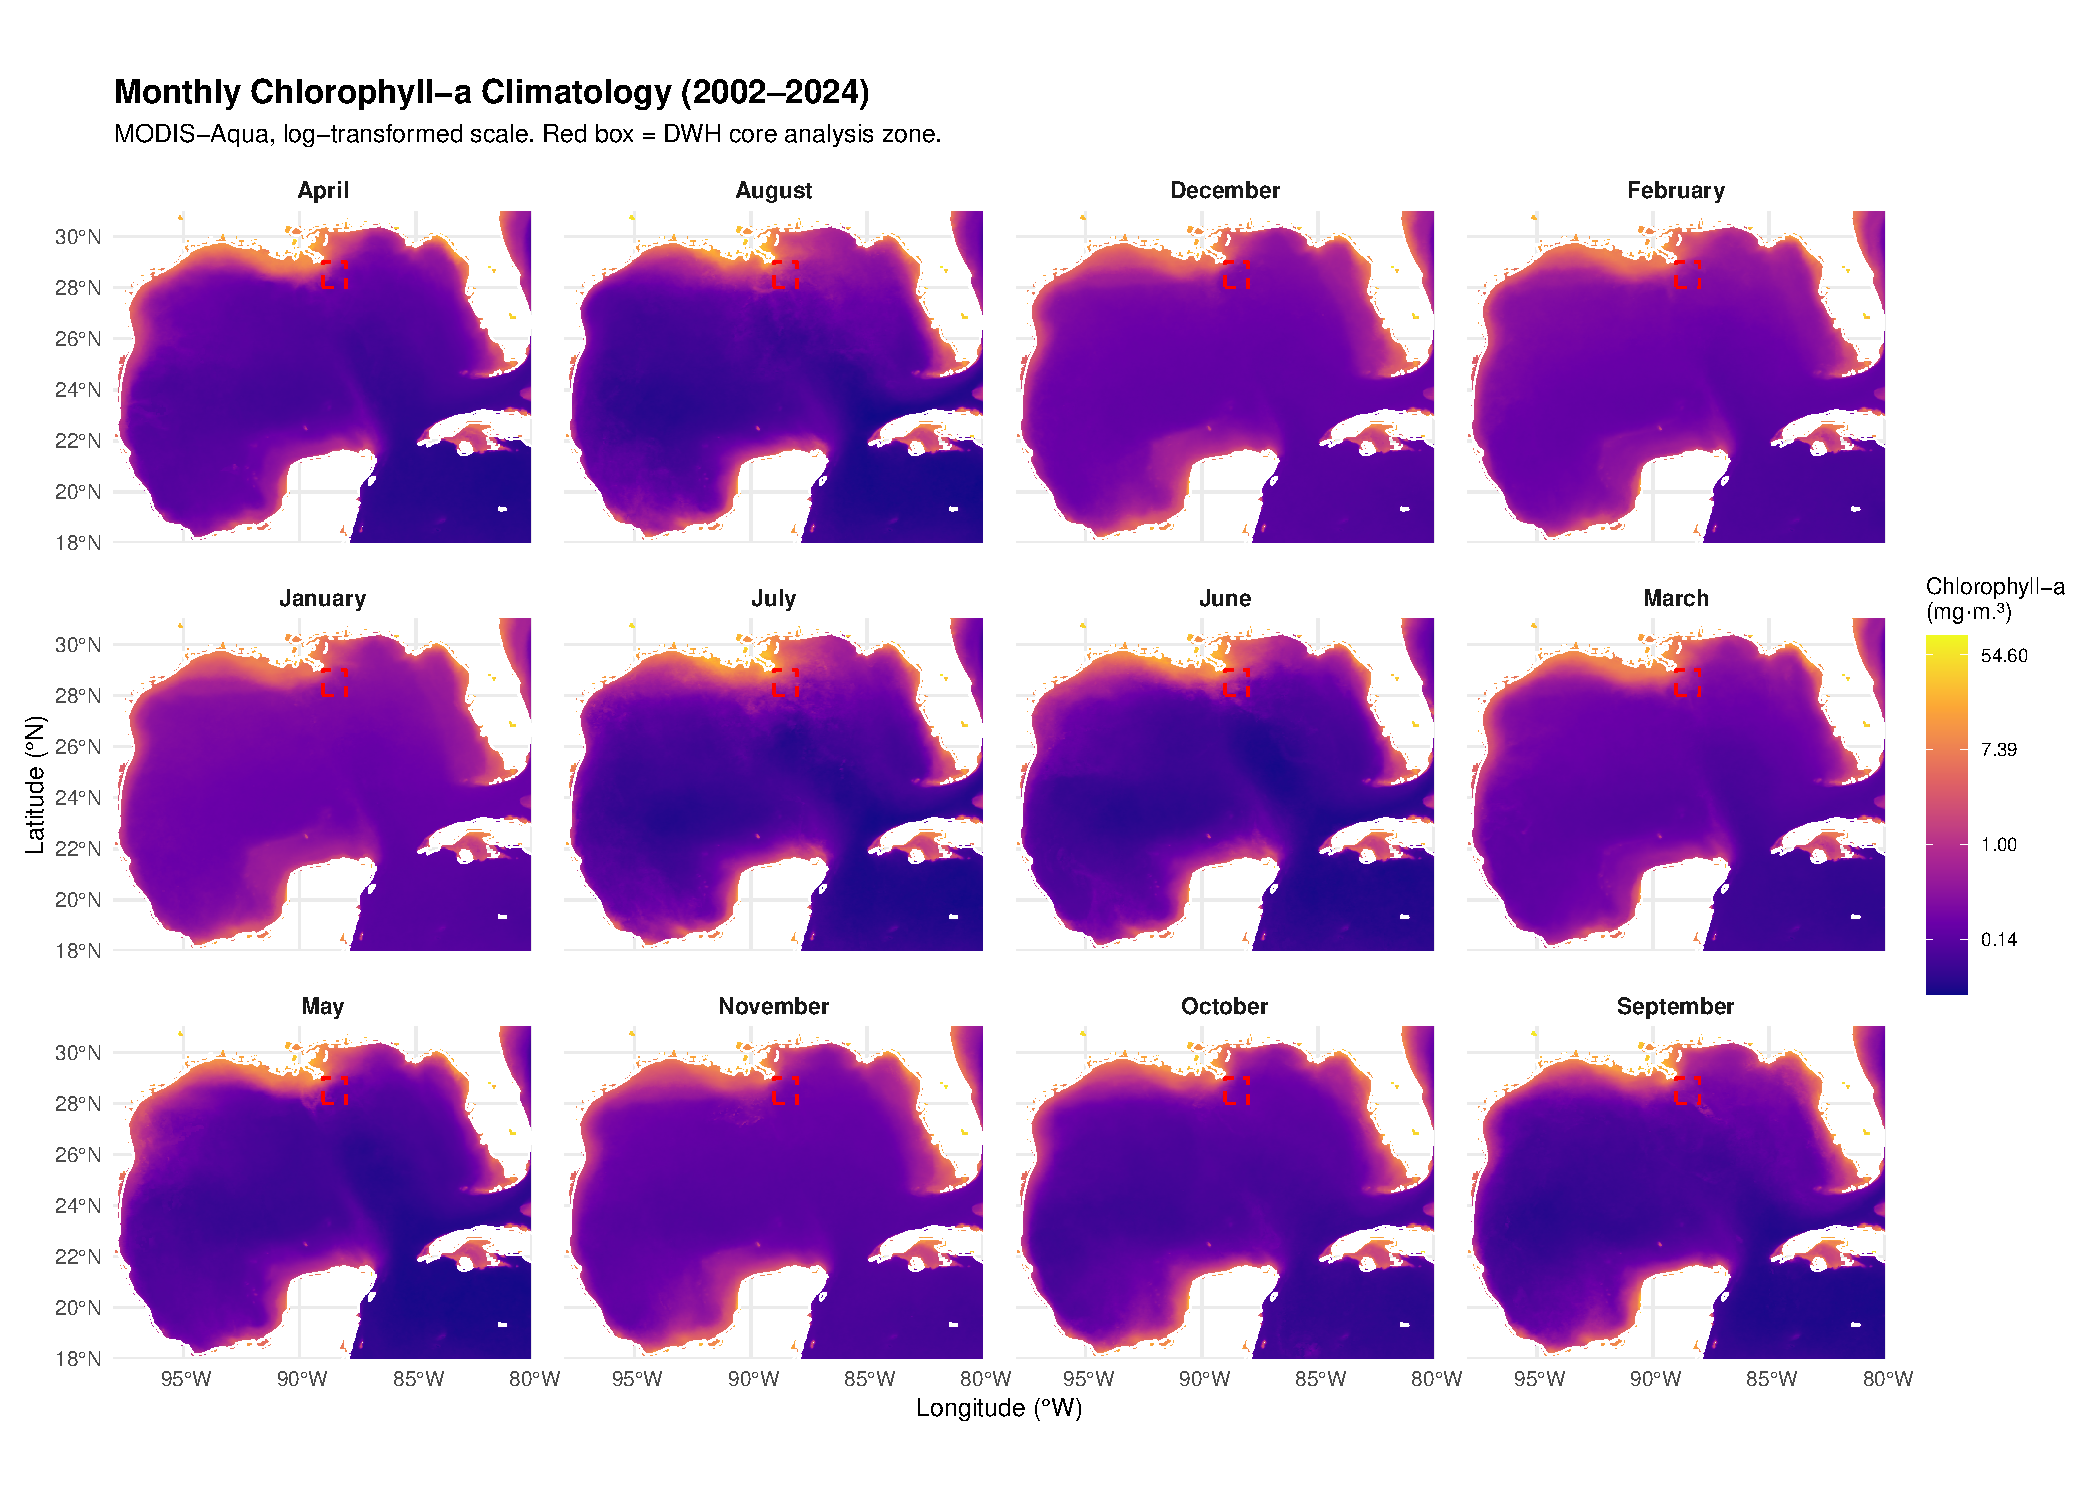
\includegraphics{figures/chlorophyll_facet.pdf}

}

\caption{Monthly chlorophyll-a climatology (mg/m³) for the Gulf of
Mexico (MODIS-Aqua, 2002--2024). Coastal productivity peaks in spring
and summer, especially along the northern shelf. Offshore regions remain
low year-round. This spatial baseline supports interpretation of
zone-based seasonal patterns and impact anomalies.}

\end{figure}%

\begin{center}\rule{0.5\linewidth}{0.5pt}\end{center}

\subsection{Zonal Seasonal Patterns}\label{zonal-seasonal-patterns}

To assess regional differences in baseline chlorophyll seasonality,
climatological means were extracted from three zones: a Deepwater
Horizon (DWH) core area (28--29°N, 88--89°W), a wider spill-influenced
region (27--30°N, 87--90.5°W), and a remote offshore control zone
(23--24°N, 91--93°W). As seen in \textbf{Figure 2}.

The DWH-wide zone (Yellow) exhibits consistently elevated chlorophyll
(\textasciitilde2.5--3.2 mg/m³), likely reflecting sustained riverine
nutrient inputs. The control zone (Blue) remains oligotrophic year-round
(\textless0.2 mg/m³). In contrast, the DWH core zone (Pink) displays a
pronounced summer peak (\textasciitilde1.3 mg/m³), suggestive of a
seasonal bloom potentially linked to ecological feedbacks or legacy
effects from the 2010 spill. These zonal distinctions highlight the
spatial heterogeneity of phytoplankton dynamics in the Gulf and justify
localised impact assessment.

\begin{figure}[H]

{\centering \includegraphics{figures/monthly_chlorophyll_climatology.pdf}

}

\caption{Seasonal chlorophyll-a climatology (mg/m³) for three spatial
zones: Deepwater Horizon core, wider spill-affected region, and offshore
control (MODIS-Aqua, 2002--2024). The DWH core shows a distinct
mid-summer peak, contrasting with the year-round productivity of the
wider shelf and the oligotrophic offshore region.}

\end{figure}%

\begin{center}\rule{0.5\linewidth}{0.5pt}\end{center}

\subsection{STL Analysis of Phytoplankton Seasonality and Disturbance
Signals}\label{stl-analysis-of-phytoplankton-seasonality-and-disturbance-signals}

To detect temporal disruptions in phytoplankton productivity linked to
the Deepwater Horizon (DWH) oil spill, seasonal-trend decomposition
using Loess (STL) was applied to log-transformed chlorophyll-a time
series across three zones: the spill's core area, a wider affected shelf
region, and an offshore control. STL decomposes time series into trend,
seasonal, and residual (remainder) components, enabling detection of
ecological anomalies beyond expected seasonal dynamics.

\begin{figure}[H]

{\centering \includegraphics[width=1\textwidth,height=\textheight]{figures/fig_stl_core.pdf}

}

\caption{STL decomposition of log-transformed chlorophyll-a in the DWH
core zone. The shaded area highlights the Deepwater Horizon spill period
(2010--2014).}

\end{figure}%

The DWH core zone (\textbf{Figure 3}) displays a marked seasonal cycle,
with mid-year chlorophyll peaks reflecting riverine and thermal controls
on phytoplankton growth. However, from 2010--2014, the seasonal
amplitude contracts and the trend component declines sharply, bottoming
out in 2012 before gradually recovering. This pattern is consistent with
documented post-spill suppression of phytoplankton biomass attributed to
reduced light penetration, hydrocarbon toxicity, and altered microbial
competition (Hu et al., 2011; Romero et al., 2015). Residual anomalies
during this period were large and variable, indicating breakdowns in
typical seasonal synchrony.

\begin{figure}[H]

{\centering \includegraphics[width=1\textwidth,height=\textheight]{figures/fig_stl_Wide.pdf}

}

\caption{STL decomposition of log-transformed chlorophyll-a in the DWH
wide zone. The shaded area highlights the Deepwater Horizon spill period
(2010--2014).}

\end{figure}%

\begin{figure}[H]

{\centering \includegraphics[width=1\textwidth,height=\textheight]{figures/fig_stl_Control.pdf}

}

\caption{STL decomposition of log-transformed chlorophyll-a in the
Control zone. The shaded area highlights the Deepwater Horizon spill
period (2010--2014).}

\end{figure}%

In contrast, the offshore control zone maintained consistent seasonal
cycles and a stable trend throughout the record (\textbf{Figure}
\textbf{3}). No comparable amplitude collapse or residual volatility was
observed, reinforcing the interpretation that the shelf response was not
a basin-wide phenomenon driven by climate variability or ENSO. The wider
spill zone (\textbf{Figure 2}) showed an intermediate response, with
modest trend depression and reduced seasonal expression from 2010--2012,
suggesting a spatial gradient in exposure intensity.

\begin{table}
\caption*{
{\large \textbf{STL Residual Summary by Zone and Time Period}} \\ 
{\small Mean and standard deviation of STL residuals (log-transformed chlorophyll-a)}
} 
\fontsize{9.0pt}{10.8pt}\selectfont
\begin{tabular*}{\linewidth}{@{\extracolsep{\fill}}llrr}
\toprule
Zone & Period & Mean Residual & SD Residual \\ 
\midrule\addlinespace[2.5pt]
Control & Post-2015 Recovery & -0.001 & 0.070 \\ 
Control & Pre-Spill (2002–2009) & -0.003 & 0.045 \\ 
Control & Spill Impact (2010–2014) & 0.007 & 0.075 \\ 
DWH Core & Post-2015 Recovery & 0.001 & 0.212 \\ 
DWH Core & Pre-Spill (2002–2009) & -0.002 & 0.192 \\ 
DWH Core & Spill Impact (2010–2014) & 0.005 & 0.201 \\ 
DWH Wide & Post-2015 Recovery & -0.001 & 0.059 \\ 
DWH Wide & Pre-Spill (2002–2009) & -0.001 & 0.062 \\ 
DWH Wide & Spill Impact (2010–2014) & 0.003 & 0.068 \\ 
\bottomrule
\end{tabular*}
\end{table}

STL decomposition of log-transformed chlorophyll-a in the DWH wide zone.
The shaded area highlights the Deepwater Horizon spill period
(2010--2014).

\textbf{Table 1} quantifies the STL remainder component (mean and
standard deviation) across three periods: \textbf{pre-spill}
(2002--2009), the \textbf{spill window} (2010--2014), and
\textbf{recovery} (post-2015). The DWH core zone exhibited the highest
residual volatility during the spill period (\textbf{SD = 0.201}), with
a persistent signal of instability extending into the recovery years
(\textbf{SD = 0.212}). These findings are consistent with ecosystem
modelling studies indicating delayed trophic recovery and prolonged
microbial succession (Li et al., 2019). The control zone, by contrast,
showed stable residuals throughout, confirming that anomalies in the
shelf zone reflect localised disruption rather than broader
oceanographic variability.

This decomposition provides strong evidence that phytoplankton seasonal
dynamics in the northern Gulf shelf were acutely disrupted by the spill
and its aftermath, supporting a view of ecosystem perturbation followed
by slow re-stabilisation. These results form a foundation for subsequent
spatial anomaly mapping and signal modelling (Section 4.4), and for
evaluating the resilience of the system in Section 4.6.

\begin{center}\rule{0.5\linewidth}{0.5pt}\end{center}

\subsection{Spatial Mapping of STL Residual Anomalies
(2010--2014)}\label{spatial-mapping-of-stl-residual-anomalies-20102014}

The spatial STL residual anomaly map (\textbf{Figure 4}) reinforces the
temporal patterns identified in Section 4.3, providing clear evidence
that phytoplankton dynamics were disrupted in a geographically
structured manner during the spill window (2010--2014). Mean residuals
were strongly positive across much of the DWH core zone and surrounding
shelf, indicating elevated chlorophyll-a levels beyond what would be
expected from seasonality or long-term trend. These anomalies are
centred near the Macondo wellhead, supporting the hypothesis that
localised ecological disturbance occurred in direct association with oil
exposure. This is consistent with previous findings that oil-induced
stratification, microbial degradation of hydrocarbons, and associated
nutrient fluxes can stimulate transient phytoplankton blooms (Hu et al.,
2011; Romero et al., 2015).

\begin{figure}[H]

{\centering \includegraphics{figures/map_stl_resid_mean_2010_14.pdf}

}

\caption{Mean STL residuals (2010--2014) across the northern Gulf of
Mexico. Red indicates anomalous chlorophyll peaks; blue indicates
suppressed phytoplankton activity. Overlays include the Deepwater
Horizon impact zones and the Macondo wellhead.}

\end{figure}%

In contrast, residuals in offshore waters and control regions were
minimal, echoing the temporal STL results which showed stable seasonal
structure and low variability outside the spill footprint. Localised
negative anomalies southwest of the core zone may reflect suppressed
productivity due to dispersed oil or reduced light availability,
highlighting the heterogeneity of ecological responses within the
impacted area. Notably, areas of highest residual magnitude align with
the previously defined DWH core zone, reinforcing the validity of our
zonal masks and supporting their use in recovery trajectory assessment.

These spatial patterns directly support the central research aim: to
determine whether phytoplankton dynamics were altered by the spill, and
to assess the extent, nature, and localisation of these effects. The STL
anomaly map visualises this disturbance footprint with high resolution,
strengthening the attribution of change to the Deepwater Horizon event.

\begin{center}\rule{0.5\linewidth}{0.5pt}\end{center}

\subsection{Event-Based Assessment of Other
Spills}\label{event-based-assessment-of-other-spills}

To assess whether the Deepwater Horizon (DWH) event represented a unique
ecological disruption or part of a broader pattern of phytoplankton
response to oil spills, chlorophyll-a time series were aligned to 127
spill events across the Gulf of Mexico between 2002 and 2025. The
resulting composite mean plot (Appendix, \textbf{Figure 9}) revealed no
consistent shift in chlorophyll levels following spill onset. Seasonal
periodicity remained dominant, with no statistically meaningful
deviation from pre-spill conditions. This suggests that, in aggregate,
Gulf oil spills have not produced systematic phytoplankton bloom or
suppression responses---potentially reflecting the limited size or
offshore dispersion of most incidents.

\begin{figure}[H]

{\centering \includegraphics{figures/mean_chlorophyll_top15_spills.pdf}

}

\caption{Mean chlorophyll-a concentration (mg·m⁻³) aligned to the 15
largest oil spills in the Gulf of Mexico (by potential volume). Time
series represent a ±4-year window centred on each spill event. Shaded
area denotes 95\% confidence interval.}

\end{figure}%

To explore whether this lack of signal masked heterogeneity among larger
events, a refined analysis focused on the 15 largest spills by maximum
potential volume. The chlorophyll-a response curve (\textbf{Figure 5})
showed slightly increased variability and a modest decline in mean
concentrations in the 6--18 months following spill onset. However, no
persistent shift or directional trend was observed. These findings are
consistent with literature highlighting the context-dependent impacts of
oil on primary producers, moderated by light attenuation, nutrient
regimes, and microbial degradation rates (Abbriano et al., 2011;
Ramirez-Llodra et al., 2011).

The absence of a consistent aggregate response among all 127 spills may
reflect both the smaller size of most events and limitations in spatial
spill metadata (Appendix, \textbf{Figure 9)}. In contrast, the top-15
analysis provides clearer insight into the conditions under which
satellite-detectable phytoplankton disruption occurs.

Taken together, the results reinforce the conclusion that
\emph{Deepwater Horizon} was ecologically exceptional, rather than
representative. Smaller and even moderately large spills appear to exert
limited or highly localised influence on satellite-detectable
phytoplankton productivity. This supports the view that system-wide
effects of oil contamination may require threshold-level disturbances,
particularly in surface extent and persistence. These findings build on
the STL decomposition and anomaly analysis (Sections 4.3--4.4), which
also demonstrated that only the DWH Core Zone exhibited a sustained and
significant phytoplankton departure from seasonal baselines.

\begin{center}\rule{0.5\linewidth}{0.5pt}\end{center}

\subsection{Phytoplankton Recovery Trajectories by
Zone}\label{phytoplankton-recovery-trajectories-by-zone}

To evaluate the ecological recovery of phytoplankton following the
Deepwater Horizon (DWH) oil spill, STL-derived trend components were
extracted from log-transformed chlorophyll-a time series across three
zones: the DWH core, wider affected shelf, and an offshore control.
\textbf{Figure 6} shows these trend trajectories from 2002 to 2024, with
the 2010 spill period shaded in red, pre-spill baseline means indicated
by dashed grey lines, and LOESS smoothed fits overlaid.

\begin{figure}[H]

{\centering \includegraphics{figures/recovery.pdf}

}

\caption{STL-derived trend components of log-transformed chlorophyll-a
by zone (2010--2024). Dashed lines represent pre-2010 baseline means.
Red shading shows the Deepwater Horizon spill period (April--July
2010).}

\end{figure}%

\begin{table}
\caption*{
{\large \textbf{Post-Spill Trend Slopes (2011--2014)}} \\ 
{\small Linear slopes fitted to STL-derived chlorophyll-a trend components}
} 
\fontsize{9.0pt}{10.8pt}\selectfont
\begin{tabular*}{\linewidth}{@{\extracolsep{\fill}}lrr}
\toprule
Zone & Trend Slope (β) & p-value \\ 
\midrule\addlinespace[2.5pt]
DWH Core & 1.93 $\times$ 10\textsuperscript{-4} & 0.636 \\ 
DWH Wide & -2.07 $\times$ 10\textsuperscript{-4} & 0.180 \\ 
Offshore Control & 4.13 $\times$ 10\textsuperscript{-4} & 0.002 \\ 
\bottomrule
\end{tabular*}
\end{table}

STL-derived trend components of log-transformed chlorophyll-a by zone
(2010--2024). Dashed lines represent pre-2010 baseline means. Red
shading shows the Deepwater Horizon spill period (April--July 2010).

The \textbf{DWH core zone} displayed a sharp decline in trend values
following the 2010 spill, reaching a minimum by mid-2012. A partial
recovery is evident between 2013 and 2018, but the STL trend plateaus
and begins to decline again after 2020. This secondary decline may
reflect long-term alterations in microbial or nutrient dynamics
following the initial post-spill response, consistent with evidence of
trophic reorganisation and decoupled carbon cycling (Parsons et al.,
2015).

The \textbf{wider DWH shelf zone} exhibited a similar though attenuated
pattern: an initial dip, followed by modest recovery, but with long-term
trends remaining below baseline. In contrast, the \textbf{offshore
control zone} showed no such disruption, instead demonstrating a gradual
and consistent recovery in chlorophyll-a trends over the entire time
series.

The overlay of LOESS curves and pre-2010 baselines highlights the
spatial disparity in ecosystem resilience. While the control zone
continued to trend upward, both impacted zones show \textbf{suppressed
or unstable recovery}, consistent with delayed microbial succession and
trophic restructuring reported in post-spill ecological modelling (Li et
al., 2019; Parsons et al., 2015). These STL-based findings reinforce
earlier results (Sections 4.3--4.5), indicating that phytoplankton
recovery in the DWH core region has remained incomplete over a decade
later, in contrast to the broader Gulf system which appears to exhibit
greater ecological stability.

To statistically evaluate recovery trajectories, linear slopes were
fitted to the STL trend components over the 2011--2014 post-spill
interval (\textbf{Figure 6}). The DWH core zone exhibited a weak
positive slope (\emph{β} = 1.93e--4, \emph{p} = 0.636), suggesting no
significant rebound in phytoplankton productivity in the four years
following the Deepwater Horizon spill. The wider affected zone showed a
slight declining trend (\emph{β} = --2.07e--4, \emph{p} = 0.18),
consistent with ongoing sub-lethal ecological disturbance. In contrast,
the offshore control zone exhibited a significant upward trend (\emph{β}
= 4.13e--4, \emph{p} = 0.002), indicating background productivity
increases unrelated to spill exposure. These findings reinforce the
visual interpretation that full recovery was not achieved in the most
exposed areas during the observed period.

While a partial trend recovery is evident by 2018 in some zones,
satellite-derived chlorophyll measures cannot confirm restoration of
species composition or ecosystem function. As such, these findings
should be interpreted as indicators of productivity stability rather
than complete ecological recovery.

\begin{center}\rule{0.5\linewidth}{0.5pt}\end{center}

\section{Discussion}\label{discussion}

This study set out to assess how oil spills---particularly the Deepwater
Horizon (DWH) disaster---impacted phytoplankton productivity and
seasonality in the Gulf of Mexico. Using time-series decomposition,
spatial anomaly detection, and event-aligned analysis, we found that
chlorophyll-a dynamics were significantly disrupted in the aftermath of
DWH, with changes persisting for several years. These disruptions were
spatially uneven, highlighting the importance of zonal analysis in
understanding ecosystem resilience to hydrocarbon disturbance.

The most striking result was the prolonged suppression of phytoplankton
productivity in the DWH core zone. STL decomposition revealed a sharp
decline in both trend and seasonal amplitude from 2010--2014, consistent
with prior findings of oil-induced toxicity and altered microbial
structure (Li et al., 2019; Parsons et al., 2015). By comparing STL
trajectories to pre-spill baselines and spatial controls, this study was
able to isolate the disturbance signal more robustly than previous work.

Although chlorophyll levels appeared to recover by \textasciitilde2015,
the trend did not return to baseline and declined again after
2020---suggesting that recovery was incomplete and unstable. This
delayed downturn illustrates the value of decomposition-based methods
over simple pre/post comparisons. Where average-difference approaches
might classify the system as `recovered', STL slope analysis revealed
more subtle but ecologically significant deviations.

Spatial heterogeneity also emerged as a key pattern. The offshore
control zone showed no comparable anomalies and trended upward, while
the wider spill zone displayed a flatter, dampened trajectory. These
differences reinforce the need to assess spill impacts across stratified
spatial units, rather than treating the Gulf as homogeneous.

The comparative analysis of 127 other Gulf oil spills further emphasised
DWH's exceptional nature. Only the largest 15 spills showed modest,
variable responses---and even these lacked consistent directionality.
This framing added an original dimension to the study, generalising
across events at a scale rarely attempted in satellite-based ecological
assessments.

While these findings offer robust insight into post-spill phytoplankton
dynamics, several limitations must be acknowledged. MODIS-Aqua
chlorophyll-a is a surface biomass proxy and cannot detect subsurface
responses such as deep chlorophyll maxima or benthic populations. In
stratified conditions, these may persist or shift undetected,
potentially underestimating ecological change.

Chlorophyll-a also does not distinguish between taxa or physiological
state. In situ studies have documented species-specific sensitivities to
oil and dispersants, affecting photosynthetic efficiency and community
composition (Almeda et al., 2013; Paul et al., 2013; Ozhan et al.,
2014). Consequently, recovery of bulk chlorophyll does not necessarily
imply functional or ecological restoration. Future work integrating
pigment or molecular indicators could address this gap.

Causality remains difficult to assign with certainty. Although spatial
controls and baseline comparisons strengthen attribution, co-occurring
drivers such as discharge or mesoscale circulation may also influence
chlorophyll patterns. Without explicit covariates, oil-related impacts
are inferred rather than modelled.

The spill comparison was further limited by metadata inconsistencies.
Many events lacked precise spatial extents, durations, or dispersant
usage records, restricting analysis of cumulative effects. This likely
contributed to the lack of detectable signal among smaller events.
Improved reporting standards would enable more comprehensive regional
assessments.

These findings contribute to growing evidence that phytoplankton
responses to oil are spatially and temporally variable. By integrating
zonal time-series decomposition with event-aligned comparisons, this
study offers a more mechanistic understanding of how productivity
responds to hydrocarbon exposure. It also underscores the importance of
assessing disturbance intensity and recovery quality---not just biomass
rebound---when evaluating ecosystem resilience.

From a data science perspective, STL decomposition and zonal trend
analysis provided a scalable, interpretable alternative to black-box
anomaly detection. Slope-based trend evaluation allowed subtle recovery
patterns to be identified---crucial in contexts where policy depends on
clear evidence of system status.

This work also reinforces the value of satellite-based ecological
monitoring, particularly in offshore regions where in situ sampling is
limited. Composite spill analysis illustrates how remote sensing can
generalise across events to detect outliers like DWH. With improved
metadata and sensor resolution, these methods could support real-time
ecosystem monitoring.

Future work could extend this approach by integrating multispectral
indicators such as nFLH or backscatter, and by incorporating
environmental covariates (e.g., discharge, salinity) to disentangle
drivers. Merging in situ or molecular data would further enable
assessment of not just recovery, but restoration of function and
composition.

\section{Conclusion}\label{conclusion}

This study investigated how large-scale oil spills---especially the
Deepwater Horizon event---have disrupted phytoplankton productivity and
seasonal structure in the Gulf of Mexico, using a data-driven approach
grounded in satellite time-series decomposition and spatial analysis.

The results demonstrate that phytoplankton responses were both spatially
uneven and temporally extended. In the DWH core zone, chlorophyll-a
trends declined sharply and did not return to baseline, indicating
incomplete recovery even a decade after the event. While smaller spills
showed little detectable impact at regional scales, this analysis
confirmed DWH as an ecological outlier with long-lasting consequences.

Methodologically, this work shows how time-series decomposition,
residual mapping, and zonal trend evaluation can offer interpretable and
scalable tools for monitoring marine ecosystem resilience. By moving
beyond binary classifications of `recovery' or `disturbance', these
techniques enable more nuanced assessments of ecological stability.

These findings carry broader significance for environmental monitoring
and disaster response. Phytoplankton are both sensitive indicators and
central actors in marine systems; understanding their disturbance
trajectories is critical. Future monitoring frameworks should integrate
remote sensing with in situ and spectral diagnostics, supported by open
and consistent spill metadata.

As oil extraction continues across vulnerable marine regions, scalable
and transparent data science methods---like those applied here---will be
vital to monitoring, interpreting, and responding to ecological
disruption in an era of intensifying marine industrialisation.

\section{Appendix:}\label{appendix}

\subsubsection{Figures:}\label{figures}

\begin{figure}[H]

{\centering \includegraphics{figures/mean_chlorophyll_all_spills.pdf}

}

\caption{Mean chlorophyll-a concentration (mg·m⁻³) aligned to all recent
oil spills in the Gulf of Mexico. Time series represent a ±4-year window
centred on each spill event. Shaded area denotes 95\% confidence
interval.}

\end{figure}%

\subsubsection{Code:}\label{code}

All code and data used in this project are available at:
\url{https://github.com/KetchupJL/university-projects/tree/main}

\subsubsection{References}\label{references}

The following references were used to inform background research,
methodology design, and interpretation of results. While some are not
explicitly cited in the main text, they contributed to the conceptual
framework and analytical direction of the study:

(Martinez, 2003; Rabalais, Turner and Wiseman, 2004; Turner, Rabalais
and Justić, 2008; Graham \emph{et al.}, 2010; Tunnell, Felder and Earle,
2010; Abbriano \emph{et al.}, 2011; Hu \emph{et al.}, 2011;
Ramirez-Llodra \emph{et al.}, 2011; McNutt \emph{et al.}, 2012; White
\emph{et al.}, 2012; Almeda \emph{et al.}, 2013, 2014; Paul \emph{et
al.}, 2013; Ozhan, Parsons and Bargu, 2014; Lewandowska \emph{et al.},
2014; Parsons \emph{et al.}, 2015; Walsh \emph{et al.}, 2015;
Muller-Karger \emph{et al.}, 2015; Romero \emph{et al.}, 2015;
Bonisoli-Alquati \emph{et al.}, 2016; O'Connor \emph{et al.}, 2016; Li
\emph{et al.}, 2019; Sutton \emph{et al.}, 2022; NOAA Office of Response
and Restoration, 2024; NASA Ocean Biology Processing Group, 2024; Lewis,
2025)

\phantomsection\label{refs}
\begin{CSLReferences}{0}{1}
\bibitem[\citeproctext]{ref-abbriano2011}
Abbriano, R. M. \emph{et al.} (2011) {`Immediate impact of the deepwater
horizon oil spill on subtidal benthic foraminifera in the northern gulf
of mexico, USA'}, \emph{Environmental Science \& Technology}, 45(19),
pp. 8787--8795.

\bibitem[\citeproctext]{ref-almeda2013interactions}
Almeda, R. \emph{et al.} (2013) {`Interactions between zooplankton and
crude oil: Toxic effects and bioaccumulation of polycyclic aromatic
hydrocarbons'}, \emph{PLOS One}, 8(6), p. e67212.

\bibitem[\citeproctext]{ref-almeda2013}
Almeda, R. \emph{et al.} (2014) {`Ingestion and sublethal effects of
physically and chemically dispersed crude oil on marine planktonic
copepods'}, \emph{Ecotoxicology}, 23(6), pp. 988--1003. doi:
\href{https://doi.org/10.1007/s10646-014-1231-6}{10.1007/s10646-014-1231-6}.

\bibitem[\citeproctext]{ref-bonisoli2016incorporation}
Bonisoli-Alquati, A. \emph{et al.} (2016) {`Incorporation of deepwater
horizon oil in a terrestrial bird'}, \emph{Environmental Research
Letters}, 11(11), p. 114023.

\bibitem[\citeproctext]{ref-graham2010oil}
Graham, W. M. \emph{et al.} (2010) {`Oil carbon entered the coastal
planktonic food web during the deepwater horizon oil spill'},
\emph{Environmental Research Letters}, 5(4), p. 045301.

\bibitem[\citeproctext]{ref-hu2011}
Hu, C. \emph{et al.} (2011) {`Did the northeastern gulf of mexico become
greener after the deepwater horizon oil spill?'}, \emph{Geophysical
Research Letters}, 38, p. L09601. doi:
\href{https://doi.org/10.1029/2011GL047184}{10.1029/2011GL047184}.

\bibitem[\citeproctext]{ref-lewandowska2014}
Lewandowska, A. M. \emph{et al.} (2014) {`Effects of sea surface warming
on marine plankton'}, \emph{Ecology Letters}, 17(5), pp. 614--623. doi:
\href{https://doi.org/10.1111/ele.12265}{10.1111/ele.12265}.

\bibitem[\citeproctext]{ref-lewis2025}
Lewis, J. (2025) {`University MSc projects repository'}.\\
url{https://github.com/KetchupJL/university-projects/tree/main}.

\bibitem[\citeproctext]{ref-li2019}
Li, Y. \emph{et al.} (2019) {`Potential influence of the deepwater
horizon oil spill on phytoplankton primary productivity in the northern
gulf of mexico'}, \emph{Environmental Research Letters}, 14(9), p.
094018. doi:
\href{https://doi.org/10.1088/1748-9326/ab3735}{10.1088/1748-9326/ab3735}.

\bibitem[\citeproctext]{ref-martinez2003}
Martinez, C. (2003) {`Northern gulf of mexico deep sea habitats 2003
mission summary'}. Available at:
\url{https://oceanexplorer.noaa.gov/explorations/03mexico/background/plan/media/summary.html}.

\bibitem[\citeproctext]{ref-mcnutt2012}
McNutt, M. K. \emph{et al.} (2012) {`Review of flow rate estimates of
the deepwater horizon oil spill'}, \emph{Proceedings of the National
Academy of Sciences}, 109(50), pp. 20260--20267. doi:
\href{https://doi.org/10.1073/pnas.1112139108}{10.1073/pnas.1112139108}.

\bibitem[\citeproctext]{ref-mullerkarger2015}
Muller-Karger, F. E. \emph{et al.} (2015) {`Natural variability of
surface oceanographic conditions in the offshore gulf of mexico'},
\emph{Progress in Oceanography}, 134, pp. 54--76. doi:
\href{https://doi.org/10.1016/j.pocean.2014.12.007}{10.1016/j.pocean.2014.12.007}.

\bibitem[\citeproctext]{ref-modis2024}
NASA Ocean Biology Processing Group (2024) {`MODIS-aqua OceanColor L3m
monthly chlorophyll-a products'}. Available at:
\url{https://oceandata.sci.gsfc.nasa.gov}.

\bibitem[\citeproctext]{ref-noaa2024}
NOAA Office of Response and Restoration (2024) {`IncidentNews oil spill
archive (2006--2021)'}. Available at:
\url{https://incidentnews.noaa.gov}.

\bibitem[\citeproctext]{ref-oconnor2016}
O'Connor, B. S. \emph{et al.} (2016) {`The role of mississippi river
discharge in offshore phytoplankton blooming in the northeastern gulf of
mexico during august 2010'}, \emph{Remote Sensing of Environment}, 173,
pp. 133--144. doi:
\href{https://doi.org/10.1016/j.rse.2015.11.004}{10.1016/j.rse.2015.11.004}.

\bibitem[\citeproctext]{ref-10.1093ux2fbiosciux2fbiu117}
Ozhan, K., Parsons, M. L. and Bargu, S. (2014) {`How were phytoplankton
affected by the deepwater horizon oil spill?'}, \emph{BioScience},
64(9), pp. 829--836. doi:
\href{https://doi.org/10.1093/biosci/biu117}{10.1093/biosci/biu117}.

\bibitem[\citeproctext]{ref-parsons2015}
Parsons, M. L. \emph{et al.} (2015) {`Phytoplankton and the macondo oil
spill: A comparison of the 2010 phytoplankton assemblage to baseline
conditions on the louisiana shelf'}, \emph{Environmental Pollution},
207, pp. 152--160. doi:
\href{https://doi.org/10.1016/j.envpol.2015.09.019}{10.1016/j.envpol.2015.09.019}.

\bibitem[\citeproctext]{ref-paul2013}
Paul, J. H. \emph{et al.} (2013) {`Toxicity and mutagenicity of gulf of
mexico waters during and after the deepwater horizon oil spill'},
\emph{Environmental Science \& Technology}, 47(17), pp. 9651--9659. doi:
\href{https://doi.org/10.1021/es401847h}{10.1021/es401847h}.

\bibitem[\citeproctext]{ref-rabalais2014}
Rabalais, N. N., Turner, R. E. and Wiseman, W. J. (2004) {`Gulf of
mexico hypoxia, a.k.a. "The dead zone"'}, \emph{Annual Review of
Ecology, Evolution, and Systematics}, 35, pp. 235--263. doi:
\href{https://doi.org/10.1146/annurev.ecolsys.35.112202.130132}{10.1146/annurev.ecolsys.35.112202.130132}.

\bibitem[\citeproctext]{ref-ramirezllodra2011}
Ramirez-Llodra, E. \emph{et al.} (2011) {`Man and the last great
wilderness: Human impact on the deep sea'}, \emph{PLOS ONE}, 6(8), p.
e22588. doi:
\href{https://doi.org/10.1371/journal.pone.0022588}{10.1371/journal.pone.0022588}.

\bibitem[\citeproctext]{ref-romero2015}
Romero, I. C. \emph{et al.} (2015) {`Hydrocarbons in deep-sea sediments
following the 2010 deepwater horizon blowout in the northeast gulf of
mexico'}, \emph{PLOS ONE}, 10(5), p. e0128371. doi:
\href{https://doi.org/10.1371/journal.pone.0128371}{10.1371/journal.pone.0128371}.

\bibitem[\citeproctext]{ref-sutton2022}
Sutton, T. T. \emph{et al.} (2022) {`The open-ocean gulf of mexico after
deepwater horizon: Synthesis of a decade of research'}, \emph{Frontiers
in Marine Science}, 9, p. 753391. doi:
\href{https://doi.org/10.3389/fmars.2022.753391}{10.3389/fmars.2022.753391}.

\bibitem[\citeproctext]{ref-tunnell2010}
Tunnell, Jr., John W., Felder, D. L. and Earle, S. A. (2010) \emph{Gulf
of mexico origin, waters, and biota: Volume 1, biodiversity}. Texas A\&M
University Press. Available at:
\url{https://www.tamupress.com/book/9781603440943/gulf-of-mexico-origin-waters-and-biota/}.

\bibitem[\citeproctext]{ref-turner2008}
Turner, R. E., Rabalais, N. N. and Justić, D. (2008) {`Gulf of mexico
hypoxia: Alternate states and a legacy'}, \emph{Environmental Science \&
Technology}, 42(7), pp. 2323--2327. doi:
\href{https://doi.org/10.1021/es071617k}{10.1021/es071617k}.

\bibitem[\citeproctext]{ref-walsh2015plankton}
Walsh, J. J. \emph{et al.} (2015) {`Plankton model of the gulf of
mexico's response to the deepwater horizon oil spill'}, \emph{Journal of
Geophysical Research: Oceans}, 120(7), pp. 3986--4008.

\bibitem[\citeproctext]{ref-white2012}
White, H. K. \emph{et al.} (2012) {`Impact of the deepwater horizon oil
spill on a deep-water coral community in the gulf of mexico'},
\emph{Proceedings of the National Academy of Sciences}, 109(50), pp.
20303--20308. doi:
\href{https://doi.org/10.1073/pnas.1118029109}{10.1073/pnas.1118029109}.

\end{CSLReferences}




\end{document}
